\section{Zadání}

Průměrné hodnocení Diplomových prací z kateder FAV

\begin{itemize}
    \item filtrace: katedry FAV (dimenzionální tabulka)
    \item agregace: průměrné hodnocení DP z kateder (faktová tabulka agregována přes obory)
\end{itemize}

\section{Osnova}

\begin{itemize}
    \item LM: Tabulky obory, studenti, abn\_diplomove\_prace, cis\_pracovist
    \item LM: analýza: Co obsahují, relevantní sloupce a jejich datové typy, další související tabulky (mimo rozsah zadání), vazby, exportovaný obrázek schématu
    \item L: Vypracování
    \item L: Postup tvorby
    \item L: založili jsme 2 Datové zdroje (in/out), založení tabulek ve výstupním datovém zdroji + skript, fyzické schéma, kontext, logické schéma, + tabulka z rekapitulace na \nolinkurl{https://www.kiv.zcu.cz/studies/predmety/ins/odi-topology.html})
    \item L: Datové modely (máme 2, pro každou výstupní tabulku), vazba dat
    \item M: popis transformace (agregace a filtrace). + obrázky obou mapování (Projects -> Mappings), podmínky filtrů, agregací a joinů.
    \item M: Obrázek konečného schéma, ukázka dat + krátký popis.
    \item M: Závěr
\end{itemize}

Samotnému vytvoření komponent ETL předcházelo založení hlavního (MASTER\_INS\_REPO) a pracovního repozitáře (TAUCHENL\_REPO).

\section{Zakládací skript}

\begin{lstlisting}[language=sql]
CREATE TABLE TRG_KATEDRY (
  KATEDRA_ID NUMERIC(16),
  KATEDRA_KOD VARCHAR(50) NOT NULL,
  KATEDRA_NAZEV VARCHAR(100),

  CONSTRAINT PK_TRG_KATEDRY PRIMARY KEY (KATEDRA_KOD)
);

CREATE TABLE TRG_HODNOCENI_DP (
  KATEDRA_KOD VARCHAR(50),
  OBOR_ID NUMERIC(10) NOT NULL,
  OBOR_NAZEV VARCHAR(55),
  HODNOCENI VARCHAR(50),

  CONSTRAINT PK_TRG_HODNOCENI_DP PRIMARY KEY (OBOR_ID),
  CONSTRAINT FK_KATEDRY_HONOCENI FOREIGN KEY (KATEDRA_KOD) REFERENCES TRG_KATEDRY (KATEDRA_KOD)
);

\end{lstlisting}

\section{Vypracování}

EM (Expectation-Maximization) algoritmus je jeden ze základních a velice efektivních přístupů, jenž je základem mnoha algoritmů strojového učení.
V konečném důsledku dochází k odhadu Gaussovských distribučních funkcí, které jsou generátory datové sady.

Samotný algoritmus se skládá ze 3 kroků:

\begin{enumerate}
    \item E-step;
    \item M-step;
    \item Výpočet chyby a návrat na bod 1.
\end{enumerate}

Před samotným výpočtem musíme stanovit prvotní odhad.
Podíváme-li se na rozložení dat (obrázek~\ref{fig:result1}), dokážeme odhadnout, že se v datech nachází 2 shluky.

\begin{figure}[htb]
    \centering
    \includegraphics[width=0.7\textwidth]{graphs/odi-mapping-trg-katedry.png}
    \caption{ODI Výstupní mapování do tabulky TRG\_KATEDRY, logické schéma}
    \label{fig:odi-mapping-trg-katedry}
\end{figure}
\FloatBarrier

\begin{figure}[htb]
    \centering
    \includegraphics[width=0.7\textwidth]{graphs/odi-mapping-trg-katedry-physical.png}
    \caption{ODI Výstupní mapování do tabulky TRG\_KATEDRY, fyzické schéma}
    \label{fig:odi-mapping-trg-katedry-physical}
\end{figure}
\FloatBarrier

\begin{figure}[htb]
    \centering
    \includegraphics[width=0.7\textwidth]{graphs/odi-mapping-trg-hodnoceni-dp.png}
    \caption{ODI Výstupní mapování do tabulky TRG\_HODNOCENI\_DP, logické schéma}
    \label{fig:odi-mapping-trg-hodnoceni}
\end{figure}
\FloatBarrier

\begin{figure}[htb]
    \centering
    \includegraphics[width=0.7\textwidth]{graphs/odi-mapping-trg-hodnoceni-dp-physical.png}
    \caption{ODI Výstupní mapování do tabulky TRG\_HODNOCENI\_DP, fyzické schéma}
    \label{fig:odi-mapping-trg-hodnoceni-physical}
\end{figure}
\FloatBarrier

\begin{figure}[htb]
    \centering
    \includegraphics[width=0.55\textwidth]{graphs/odi-transformation-components.png}
    \caption{ODI nabídka komponent}
    \label{fig:odi-transformation-components}
\end{figure}
\FloatBarrier

\begin{figure}[htb]
    \centering
    \includegraphics[width=0.3\textwidth]{graphs/trg-model.png}
    \caption{Výstupní schéma}
    \label{fig:trg-model}
\end{figure}
\FloatBarrier

\begin{figure}[htb]
    \centering
    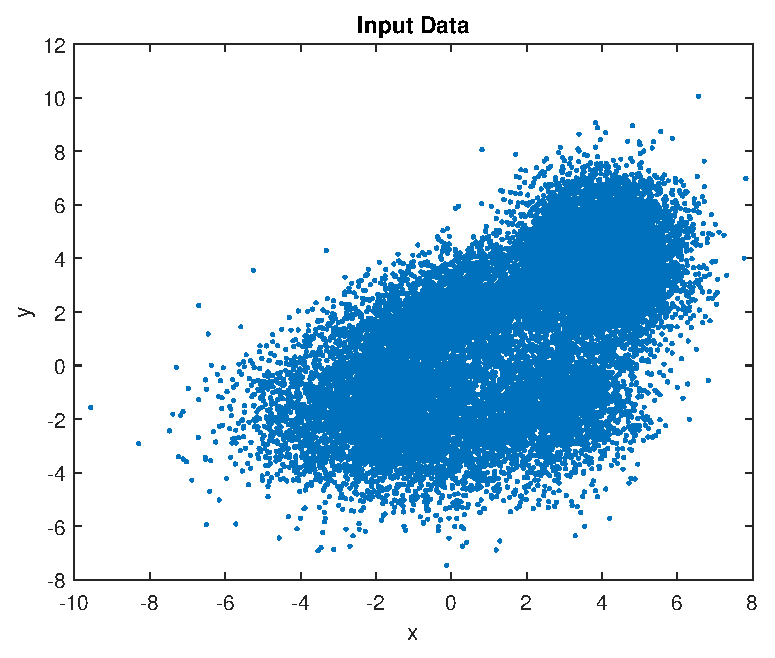
\includegraphics[width=0.55\textwidth]{graphs/fig1.eps}
    \caption{Vstupní data}
    \label{fig:result1}
\end{figure}
\FloatBarrier

Předpokládám symetričnost prvků Gaussovské směsi, tudíž \( \Sigma = I \), protože její asymetričnost sice mohu předpokládat, ale nedokázal bych odhadnout jakým způsobem je asymetrická.
Středy shluků \( \mu_1, \mu_2 \) byly určeny algoritmem \textit{k-means}, tudíž prvotní odhad je i řešením ke kterému bychom měli po několika iteracích dojít.
Počáteční váhy Normálních rozdělení byly zvoleny jako \( \frac{1}{\text{počet tříd}} \pm 0.1 \), protože z obrázku vyplývá, že váha každé ze tříd bude rozdílná.

Výpočet byl proveden dvěma způsoby.
První výpočet je kontrolní, pouze s využitím funkcionalit softwaru MATLAB.
Výsledek tohoto výpočtu je na obrázku~\ref{fig:result2}.

\begin{figure}[htb]
    \centering
    \includegraphics[width=0.55\textwidth]{graphs/fig2.eps}
    \caption{Výsledné rozdělení dat dle nativního EM algorimu}
    \label{fig:result2}
\end{figure}
\FloatBarrier

Graf~\ref{fig:result3} zobrazuje výsledek po výpočtu implementovaným E-M algoritmem.

\begin{figure}[htb]
    \centering
    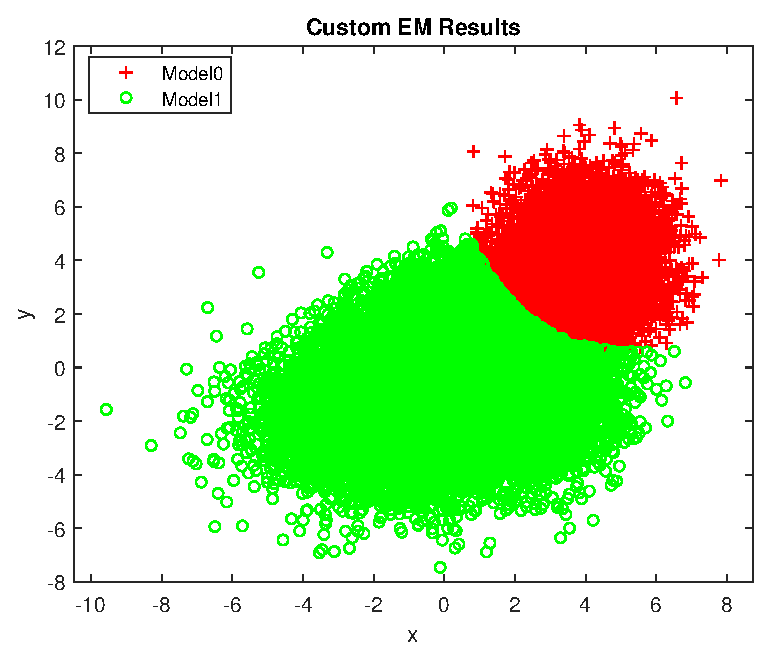
\includegraphics[width=0.55\textwidth]{graphs/fig3.eps}
    \caption{Výsledné rozdělení dat dle implementovaného E-M algorimu}
    \label{fig:result3}
\end{figure}
\FloatBarrier

Tabelované hodnoty dle zadání jsou v tabulce~\ref{table:table1}.

\begin{table}[htb]
    \centering

    \begin{tabular}{lrcc}
        \toprule

        Iterace & Chyba     & \( \mu_1 \)       & \( \mu_2 \)       \\ \midrule
        1       & 0.0537    & [-0.4510 -1.2142] & [3.5411 3.6698]   \\
        2       & 0.3032    & [-0.3409 -1.1012] & [3.6216 3.7909]   \\
        3       & 0.2412    & [-0.2684 -0.9977] & [3.7013 3.8736]   \\
        4       & 0.1674    & [-0.2227 -0.9211] & [3.7617 3.9233]   \\
        5       & 0.1226    & [-0.1919 -0.8618] & [3.8086 3.9536]   \\
        6       & 0.0952    & [-0.1675 -0.8166] & [3.8453 3.9777]   \\
        7       & 0.0638    & [-0.1499 -0.7863] & [3.8689 3.9941]   \\
        8       & 0.0411    & [-0.1373 -0.7663] & [3.8831 4.0043]   \\
        9       & 0.0245    & [-0.1304 -0.7548] & [3.8921 4.0107]   \\
        10      & 0.0123    & [-0.1274 -0.7487] & [3.8970 4.0131]   \\
        11      & 0.0037    & [-0.1262 -0.7470] & [3.8982 4.0143]   \\
        12      & 0.0025    & [-0.1253 -0.7459] & [3.8989 4.0149]   \\
        13      & 0.0007    & [-0.1252 -0.7455] & [3.8993 4.0150]   \\
          
        \bottomrule
    \end{tabular}

    \caption{Tabulované hodnoty parametrů pro každou iteraci}
    \label{table:table1}
\end{table}
\FloatBarrier

Závislost chyby na počtu iterací je v grafu~\ref{fig:result4}.
Prvotní \enquote{velmi} přesný odhad (tedy malá chyba) je způsobena tím, že první odhad je vypočtem algoritmem \textit{k-means}.
Po následné reevaluaci rozložení dat ve shlucích jsou středy přepočteny a jelikož se jedná o teprve druhý krok algoritmu, tak tím hohužel znepřesněny.

\begin{figure}[htb]
    \centering
    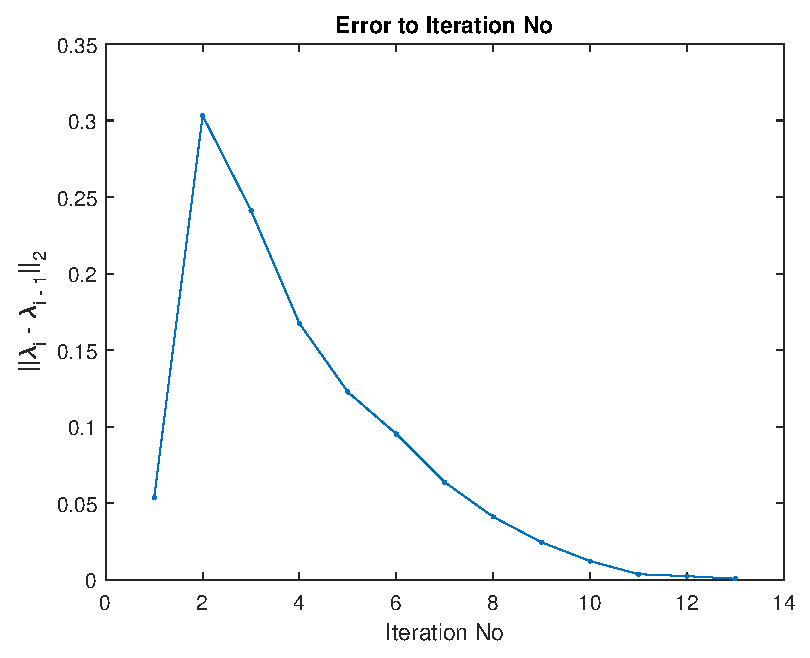
\includegraphics[width=0.55\textwidth]{graphs/fig4.eps}
    \caption{Hodnota chyby v každém uplynulém iteračním kroce}
    \label{fig:result4}
\end{figure}
\FloatBarrier

\section{Závěr}

sdfsfd
